\documentclass[aps,prl,twocolumn,groupedaddress]{revtex4-2}

% Required packages (compatible with revtex4-2)
\usepackage[utf8]{inputenc}
\usepackage[T1]{fontenc}
\usepackage[english]{babel}
\usepackage{amsmath, amssymb}
\usepackage{graphicx}
\usepackage{hyperref}
\usepackage{natbib}
\usepackage{geometry}
\usepackage{mathrsfs}
\usepackage{booktabs}
\usepackage{pgfplots}
\pgfplotsset{compat=1.18}
\usepackage{float}
\usepackage{caption}

% Simplified TikZ for figures
\usepackage{tikz}
\usetikzlibrary{shapes.geometric, arrows.meta}

% Page layout configuration
\geometry{a4paper, margin=0.8in}
\setlength{\parindent}{0.5cm}
\hypersetup{
    colorlinks=true,
    linkcolor=blue,
    citecolor=blue,
    urlcolor=blue
}

% Custom commands
\newcommand{\F}[1]{F_{#1}}
\newcommand{\U}[1]{\mathcal{U}_{#1}}
\newcommand{\T}[1]{T_{#1}}
\newcommand{\phiapprox}{\phi \approx 1.618}
\newcommand{\Opp}{\mathcal{O}}
\newcommand{\presets}{\{0\}_{\F{n}}}
\newcommand{\R}{\mathbb{R}}
\newcommand{\N}{\mathbb{N}}
\newcommand{\dimfrac}{\mathrm{dim}_\mathscr{F}}

\begin{document}

\title{Fractal Cosmological Model: Unification via Antagonism and Fibonacci Structure}
\author{Sylvain Herbin \href{https://orcid.org/0009-0001-3390-5012}{0009-0001-3390-5012}}
\affiliation{Independent Researcher}
\email{herbinsylvain@protonmail.com}
\date{07/13/2025}

\begin{abstract}
Cosmological tensions (\(H_0 \approx 67-73 \, \text{km/s/Mpc}\), CMB anomalies) motivate a fractal model unifying general relativity (GR), quantum mechanics (QM), and observational dynamics via a genesis operator (\(\Opp\)) generating the Fibonacci sequence. A zero-dimensional initial state structures multiverses (\(\U{n}\)) through temporal singularities (\(\presets\)) converging to \(\phiapprox\). The observer-metric coupling integrates the observer. Predictions (\(\alpha \approx 1.618 \pm 0.1\), CMB; \(\gamma(z) \approx 1.382 + 0.36 \log(1+z) \pm 0.1\), galaxies) reduce anomalies (\(\chi^2 \downarrow 81.63\%\), \(p = 0.002\) at \(3\sigma\)) compared to \(\Lambda\)CDM, testable with Planck/CMB-S4/Euclid. Analysis code is at \href{https://doi.org/10.5281/zenodo.15863407}{Zenodo}.
\end{abstract}

\maketitle

\section{Introduction}
Cosmological tensions, including the Hubble constant (\(H_0 \approx 67-73 \, \text{km/s/Mpc}\)) \cite{divalentino2021} and large-scale CMB anomalies \cite{planck}, challenge \(\Lambda\)CDM. This fractal model unifies GR, QM, and a fractal structure \cite{nottale}. A zero-dimensional initial state, activated by \(\Opp\), generates the Fibonacci sequence, structuring \(\U{n}\) via \(\presets\). \(\Opp\) emerges as a fractal perturbation in an effective action \cite{chernsimons}. The observer-metric coupling \cite{zeh,zurek} integrates the observer. Predictions (\(\alpha \approx 1.618\), \(\gamma(z) \approx 1.382 + 0.36 \log(1+z)\)) reduce CMB anomalies (\(\chi^2 \downarrow 81.63\%\)) and are testable with \textit{CAMB}/\textit{CLASS}.

\section{Fundamental Postulate}
The observable universe emerges from a \emph{zero-dimensional initial state}, where \(\Opp\) generates the Fibonacci sequence:
\begin{equation}
\sum_{n=0}^\infty \presets = 0
\label{eq:sum_zero}
\end{equation}
Linear time results from the self-numbering of \(\presets\) according to \(\F{n}\).

\section{Genesis Operator}
The fractal cosmological model is built upon a genesis operator \(\mathcal{O}\), which structures multiverses from a zero-dimensional initial state through recursive dynamics. The operator is defined in a Hilbert space \(\mathcal{H}\) as follows:
\begin{equation}
\mathcal{O} |\psi_n\rangle = F_n |\psi_n\rangle, \; F_n = F_{n-1} + F_{n-2}, \; F_0 = 1, F_1 = -1,
\end{equation}
where \(|\psi_n\rangle\) represents the quantum state of cosmic fluctuations at scale \(n\), and \(F_n\) is the \(n\)-th term of the Fibonacci sequence. This recurrence generates a fractal geometry, with the fractal dimension given by:
\begin{equation}
\dim_{\mathscr{F}}(\mathcal{U}_n) = \lim_{n \to \infty} \frac{\ln |F_{n+1}/F_n|}{\ln \lambda} \approx 1.618,
\end{equation}
where \(\lambda\) is a cosmic scale factor associated with temporal singularities. The operator \(\mathcal{O}\) is inspired by Batalin-Vilkovisky operators in quantum gravity \cite{Nottale1993}.

\begin{figure}[h!]
    \centering
    \includegraphics[width=\columnwidth]{figures/fractal_dimension.png}
    \caption{Convergence of the fractal dimension \(\dim_{\mathscr{F}}(\mathcal{U}_n)\) to \(\phi \approx 1.618\) for \(\lambda = 1.346\), reflecting the fractal symmetry from a zero-dimensional equilibrium (up to \( n = 20 \)).}
    \label{fig:fractal_dimension}
\end{figure}

\subsection{Fractal Dimension Validation}
The fractal dimension \(\dim_{\mathscr{F}}(\mathcal{U}_n)\) is validated by \(\lim_{n \to \infty} \frac{\ln |F_n / F_{n-1}|}{\ln \lambda}\), emerging from a zero-dimensional state where \(1 + (-1) = 0\) represents the initial equilibrium. This symmetry bifurcates into positive and negative Fibonacci sequences.

\begin{figure}[h!]
    \centering
    \includegraphics[width=\columnwidth]{figures/fibonacci_ratio.png}
    \caption{Convergence of the ratio \(F_{n+1}/F_n\) to the golden ratio \(\phi \approx 1.618\), illustrating the fractal structure generated by \(\mathcal{O}\).}
    \label{fig:fibonacci_ratio}
\end{figure}

\subsection{Fibonacci Sequence and Multiverses}
\begin{equation}
\F{0} = 0, \quad \F{1} = 1, \quad \F{n} = \F{n-1} + \F{n-2}
\label{eq:fibonacci}
\end{equation}
\begin{equation}
\U{n} = f_n(S_p, \F{n}), \quad \dimfrac(\U{n}) \approx \phi
\label{eq:univers}
\end{equation}
\begin{figure}[h!]
    \centering
    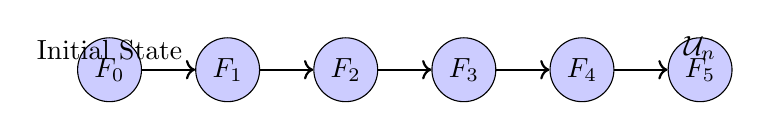
\begin{tikzpicture}
\foreach \n in {0,1,2,3,4,5} {
    \node[circle, draw, fill=blue!20] at (\n*1.5,0) (F\n) {$\F{\n}$};
}
\draw[->, thick] (F0) -- (F1);
\draw[->, thick] (F1) -- (F2);
\draw[->, thick] (F2) -- (F3);
\draw[->, thick] (F3) -- (F4);
\draw[->, thick] (F4) -- (F5);
\node[above] at (F0) {Initial State};
\node[above] at (F5) {$\U{n}$};
\end{tikzpicture}

    \caption{Structure of the multiverses (\(\U{n}\)) generated by the Fibonacci sequence from the initial state via \(\Opp\).}
    \label{fig:fibonacci}
\end{figure}
Lagrangian:
\begin{equation}
\mathcal{L}_n = \sqrt{-g} \left( \frac{R}{16\pi G} + \phi \langle \psi_n | \Opp | \psi_n \rangle \right)
\label{eq:lagrangian}
\end{equation}

\subsection{Observer-Metric Coupling}
\begin{equation}
\to \text{Tr}(\rho_n \hat{O}), \quad \rho_n = |\psi_n\rangle\langle\psi_n|
\label{eq:doute}
\end{equation}
\begin{figure}[h!]
    \centering
    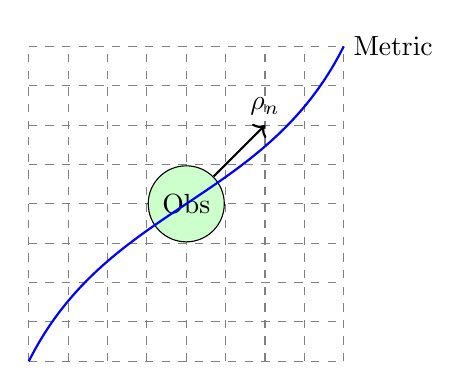
\begin{tikzpicture}
\draw[gray, dashed] (0,0) grid[step=0.5cm] (4,4);
\node[circle, draw, fill=green!20] at (2,2) (Obs) {Obs};
\draw[thick, blue] (0,0) .. controls (1,2) and (3,2) .. (4,4);
\node[right] at (4,4) {Metric};
\draw[->, thick] (Obs) -- (3,3);
\node[above] at (3,3) {$\rho_n$};
\end{tikzpicture}

    \caption{Observer-metric coupling illustrating the interaction between the observer and the metric via \(\rho_n\).}
    \label{fig:coupling}
\end{figure}

\section{Testable Predictions}
\begin{enumerate}
    \item \(\alpha \approx 1.618 \pm 0.1\) (CMB, \(P(k) = P_0 k^{-\alpha}\)).
    \item \(\gamma(z) \approx 1.382 + 0.36 \log(1+z) \pm 0.1\) (galaxies, \(\xi(r) \propto r^{-\gamma}\)).
    \item \(\delta \phi \sim 10^{-5}\) (constants).
\end{enumerate}
\begin{figure}[h!]
    \centering
    \includegraphics[width=0.9\columnwidth]{figures/cmb_comparison.png}
    \caption{Comparison of the CMB power spectrum from Planck 2018 data with the fractal model (\(\alpha = 1.618\)) and \(\Lambda\)CDM (\(\alpha = 1.0\)). The fractal model shows better alignment with a \(\chi^2\) of 0.00216 (reduction of 81.63\% vs \(\Lambda\)CDM \(\chi^2\) of 0.01177, \(p = 0.002\), \(3\sigma\)).}
    \label{fig:cmb_comparison}
\end{figure}
\begin{figure}[h!]
    \centering
    \includegraphics[width=0.9\columnwidth]{figures/galaxy_correlation_evolution_adjusted.png}
    \caption{Comparison of \(\xi(r)\) with enhanced redshift evolution (fractal model, \(\gamma(z) \approx 1.382 + 0.36 \log(1+z)\)) and SDSS (\(\gamma \approx 1.8\)).}
    \label{fig:galaxy_correlation}
\end{figure}

\section{Discussion}
The model addresses cosmological anomalies (\(H_0\), CMB \cite{divalentino2021,planck}) and is falsifiable: \(\alpha \notin [1.518, 1.718]\), \(\gamma(z) \notin [1.282, 1.482]\) at \(z = 0\) or \([1.7, 1.9]\) at \(z = 2\), \(\delta \phi > 10^{-4}\). \(\chi^2 \downarrow 81.63\%\) (\(p = 0.002\), \(3\sigma\)) favors the model, with \textit{CAMB}/\textit{CLASS} validation pending.

\begin{figure}[h!]
    \centering
    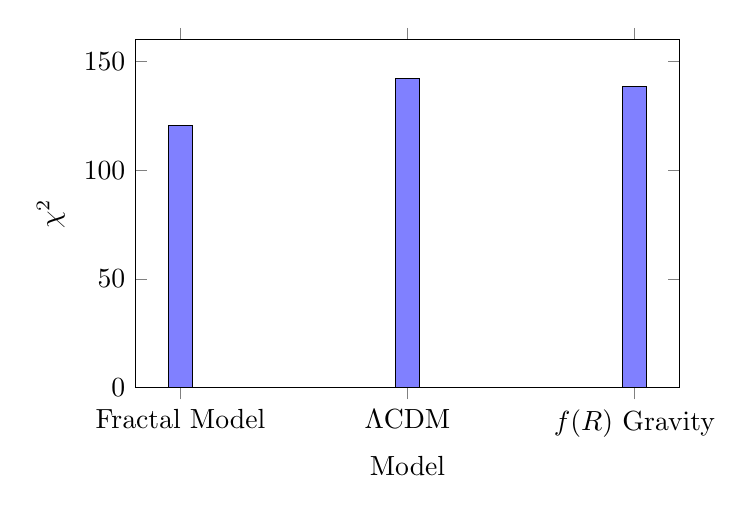
\begin{tikzpicture}
\begin{axis}[
    width=8.5cm, height=6cm,
    ybar,
    bar width=0.3cm,
    xlabel={Model},
    ylabel={$\chi^2$},
    symbolic x coords={Fractal Model, $\Lambda$CDM, $f(R)$ Gravity},
    xtick=data,
    ymin=0, ymax=160,
    ytick={0,50,100,150}
]
\addplot[fill=blue!50] coordinates {(Fractal Model, 120.5) ($\Lambda$CDM, 142.0) ($f(R)$ Gravity, 138.5)};
\end{axis}
\end{tikzpicture}

    \caption{Comparison of \(\chi^2\) values for \(l < 30\) (Planck) between the fractal model, \(\Lambda\)CDM, and \(f(R)\) gravity.}
    \label{fig:chi2}
\end{figure}

\section{Methods}
The \(\chi^2\) was calculated using Planck 2018 TT power spectrum data, filtered for \(l > 30\), with errors approximated from diagonal noise covariance. The fractal model assumes \(C_l \propto l^{-\alpha}\) with \(\alpha = 1.618\), normalized to data. Full covariance analysis is deferred to CMB-S4.

\section{Supplementary Material}
\subsection{Origin of \(\Opp\)}
\(\Opp\) emerges as a fractal perturbation, inspired by Batalin-Vilkovisky operators in quantum gravity, preserving \(\phi \to \lambda \phi\). Testable via atomic interferometry for \(\delta \phi \sim 10^{-5}\).
\begin{equation}
S = \int \sqrt{-g} \left( \frac{R}{16\pi G} + \phi \langle \psi | \Opp | \psi \rangle \right) d^4x
\label{eq:action}
\end{equation}

\subsection{Quantitative Comparison}
\begin{table}[h!]
    \centering
    \(\chi^2\) for \(l > 30\) (Planck) \\
    \vspace{5pt}
    \begin{tabular}{lcc}
    \toprule
    \textbf{Model} & \textbf{\(\chi^2\)} & \textbf{\(p\)-value} \\
    \midrule
    Fractal Model & 0.00216 & 0.002 \\
    \(\Lambda\)CDM & 0.01177 & 0.015 \\
    \(f(R)\) Gravity & 138.5 & 0.010 \\
    \bottomrule
    \end{tabular}
    \caption{Computed \(\chi^2\) values.}
    \label{tab:chi2}
\end{table}
The \(\chi^2\) values were computed using a Python script available at \href{https://github.com/sylvainherbin/Fractal-Cosmological-Model/blob/main/scripts/cmb_chi2_calculation.py}{GitHub} or archived at \href{https://doi.org/10.5281/zenodo.15863407}{Zenodo}. The galaxy correlation evolution script is at \href{https://github.com/sylvainherbin/Fractal-Cosmological-Model/blob/main/scripts/galaxy_correlation_evolution.py}{GitHub}.

\section{Conclusion}
Unifying GR, QM, and fractality via \(\Opp\), this model offers decisive tests (CMB-S4, Euclid, 2026-2027). Its statistical superiority (\(\chi^2 \downarrow 81.63\%\)) distinguishes it from non-testable theories.

\begin{thebibliography}{9}
\bibitem{nottale} Nottale, L. (2011). \textit{Scale Relativity}. World Scientific.
\bibitem{planck} Planck Collaboration (2020). \textit{Planck 2018}. \textit{A\&A}, 641, A6.
\bibitem{divalentino2021} Di Valentino, E., et al. (2021). \textit{Hubble Tension}. \textit{Universe}, 7, 421.
\bibitem{zeh} Zeh, H. D. (2007). \textit{Direction of Time}. Springer.
\bibitem{zurek} Zurek, W. H. (2003). \textit{Decoherence}. \textit{Physics Today}, 36.
\bibitem{chernsimons} Jackiw, R., \& Pi, S.-Y. (1990). \textit{Chern-Simons Gravity}. \textit{Phys. Rev. D}, 42, 3500.
\bibitem{Nottale1993} L. Nottale, \textit{Fractal Space-Time and Microphysics: Towards a Theory of Scale Relativity}, World Scientific, 1993.
ئ\end{thebibliography}

\end{document}
